\documentclass[a4paper, 11pt]{article}
\usepackage{geometry}
\usepackage{setspace}
\usepackage{amsmath}
\usepackage{graphicx}
\usepackage{caption}
\usepackage{indentfirst}
\usepackage{amssymb}
\usepackage{float}

\graphicspath{ {./images/} }
\geometry{left=2.5cm, right=2.5cm, top=2.5cm, bottom=2.5cm}

\begin{document}	
	\title{Exercise \# 1. Numerical methods for ODES. }
	\author{{\small Alexandre Rodrigues (2039952)}}
	\date{\today}
	
	\maketitle
	
		\section*{Question 1}
			
			The Simpson's method is a method to solve Ordinary Differential Equations (ODEs) defined by
			\begin{equation}
				y_{n+2} = y_n + \frac{h}{3}\left( f_n + 4 f_{n+1} + f_{n+2} \right).
			\end{equation}
	
			The ODE to solve in this question is 
			\begin{equation}
				y'(t) = -5y(t) = f(t_n,y_n),	\qquad y(0) =1.
			\end{equation}
			
			To solve this ODE with the Simpson's method the value of $ y_1 = y(h) $ also needs to be determined.
			
			One approach is to use the Forward Euler method, in the following way:
			\begin{equation}
				y_1 = y(t = h) = y(0) + h f(0,y(0))
			\end{equation}
		
			Another method one can use is the 4-th order Runge Kutta method, given by
			\begin{align}
				k_1 &= f(0,y(0)) \\
				k_2 &= f\left(\frac{h}{2},y(0) + \frac{h}{2}k_1\right) \\
				k_3 &= f\left(\frac{h}{2},y(0) + \frac{h}{2}k_2\right)\\
				k_4 &= f\left(h,y(0) + hk_3\right) \\
				y_1 = y(t = h) &= y(0) + \frac{h}{6} \left(k_1 + 2k_2 + 2k_3 + k_4 \right)
			\end{align}
					
			The results of the computations were then compared with the exact solution
			\begin{equation}
				y(t) = e^{-5t},
			\end{equation}
			to understand the influence of the methods used to compute $y(t=h)$.
			
			\begin{figure}[H]
				\centering
				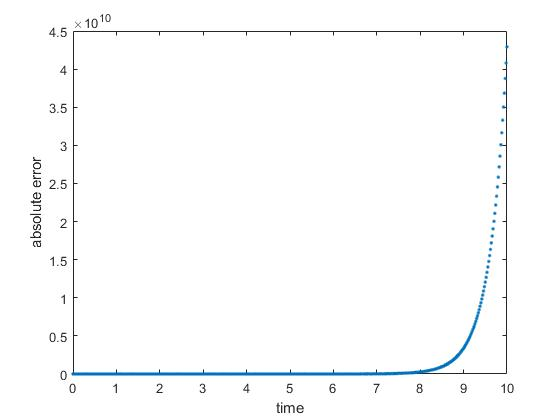
\includegraphics[width=.6\linewidth]{ex1_fe.jpg}
				\caption{Absolute error in function of time using the Forward Euler method to compute $y(t=h)$}
				\label{fig:ex1_fe}
			\end{figure}
			
			The final error when using the Forward Euler to compute $y(t=h)$ is $4.2916 \times 10^{10}$.
			
			\begin{figure}[H]
				\centering
				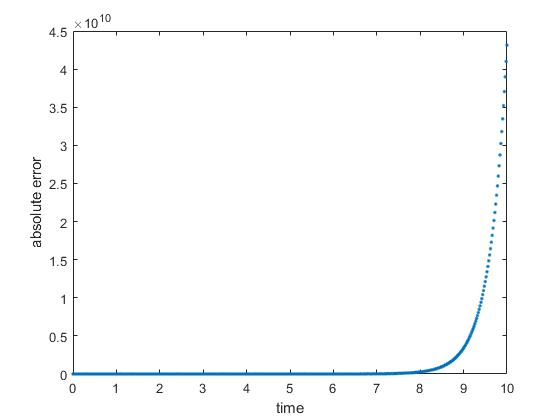
\includegraphics[width=.6\linewidth]{ex1_rk4.jpg}
				\caption{Absolute error in function of time using the RK4 method to compute $y(t=h)$}
				\label{fig:ex1_rk4}
			\end{figure}
			
			The final error when using the 4-th order Runge Kutta method to compute $y(t=h)$  is $4.3146 \times 10^{10}$.
			
			The Simpson's method has an empty stability region, which explains the large final error.
			The FE calculation for $y(t=h)$ is better then the RK4 calculation given the lower final error.
			This is, although, not very relevant because the difference is about $ 0.5 \times 10^{-10} \% $.
			
			\section*{Question 2}
			
			The method used for this question is the 4-th order Runge Kutta method defined by
			\begin{align}
				k_1 &= f(t_n,y_n) \\
				k_2 &= f\left(t_n+\frac{h}{2},y_n + \frac{h}{2}k_1\right) \\
				k_3 &= f\left(t_n+\frac{h}{2},y_n + \frac{h}{2}k_2\right)\\
				k_4 &= f\left(t_n+h,y_n + hk_3\right) \\
				y_{n+1} &= y_n + \frac{h}{6} \left(k_1 + 2k_2 + 2k_3 + k_4 \right)
			\end{align}
		
			The Ordinary Differential Equation to solve in this question is 
			\begin{equation}
				y'(t) = -10y^2(t) = f(t_n,y_n),	\qquad y(0) =1.
			\end{equation}
		
			The exact solution is 
			\begin{equation}
				y(t) = \frac{1}{10t + 1},
			\end{equation}
			which will be used to compute the error as the difference between the exact and the experimental solutions.
			
			\begin{figure}[H]
				\centering
				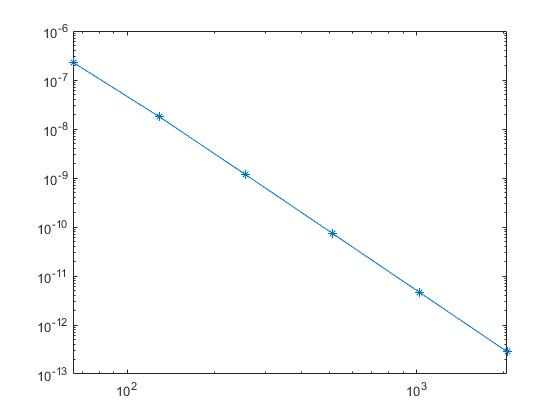
\includegraphics[width=.6\linewidth]{ex2.jpg}
				\caption{LogLog plot of the error as a function of the number of steps.}
				\label{fig:ex2}
			\end{figure}
			
			\begin{table}[H]
				\centering
				\begin{tabular}{c|c}
					\textbf{h}& \textbf{error}   \\ \hline
					$ 3.125000\times 10^{-2} $ & $ 2.291844\times 10^{-7} $ \\ \hline
					$ 1.562500\times 10^{-2} $ & $ 1.785763\times 10^{-8} $ \\ \hline
					$ 7.812500\times 10^{-3} $ & $ 1.160234\times 10^{-9} $ \\ \hline
					$ 3.906250\times 10^{-3} $ & $ 7.312862\times 10^{-11} $ \\ \hline
					$ 1.953125\times 10^{-3} $ & $ 4.579586\times 10^{-12} $ \\ \hline
					$ 9.765625\times 10^{-4} $ & $ 2.863750\times 10^{-13} $ \\ \hline	
				\end{tabular}
				\caption{Final error for each value of $h$}
				\label{table:ex2}
			\end{table}
		
			In figure \ref{fig:ex2} and table \ref{table:ex2}, you can see the clear decrease in the final error with the increase of the number of steps (halving $h$) as expected in theory.		
		
		\section*{Question 3}
			\subsection*{BDF2 derivation}
			
				The usual form of the ODE:
				\begin{align}
					y'(t) &= f(t, y(t)) \\
					y(t_0) &= y_0
				\end{align}
			
				Writing this ODE on a point $t_{n+k}$:
				\begin{equation}
					y'(t_{n+k}) = f(t_{n+k}, y_{n+k}) 
				\end{equation}
			
				The general expression of the Backward Differentiation Formulas is:
				\begin{equation}
					\sum_{j=0}^{k}\alpha_j y_{n+j} = h \beta_k f(t_{n+k}, y_{n+k}) \quad \beta_{k-1} = \ldots = \beta_0 = 0.
				\end{equation}
			
				To obtain the BDF2 formula I will interpolate the function $y(t)$ using the points $(t_{n}, y_{n})$, $(t_{n+1}, y_{n+1})$,$(t_{n+2}, y_{n+2})$.
				The resulting polynomial $P(t)$ is
				\begin{equation}
					P(t) = y_n \frac{(t - t_{n+1})(t - t_{n+2})}{2h^2} + y_{n+1} \frac{(t - t_n)(t - t_{n+2})}{-h^2} + y_{n+2} \frac{(t - t_n)(t - t_{n+1})}{2h^2}
				\end{equation}
			
				$P'(t_{n+2})$ is then used to approximate $y'(t_{n+2})$
				\begin{equation}
					P'(t) = \frac{1}{2h^2} y_n(t-t_{n+1}) - \frac{1}{h^2} y_{n+1}(t-t_{n}) + \frac{1}{2h^2} y_{n+2}[(t-t_{n})+(t-t_{n+1})] + terms \ (t-t_{n+2})
				\end{equation}
			
				The terms with $t-t_{n+2}$ are omitted because they are null for $t = t_{n-2}$.
				\begin{align}
					P'(t_{n+2}) &= \frac{1}{2h^2} y_n(t_{n+2}-t_{n+1}) - \frac{1}{h^2} y_{n+1}(t_{n+2}-t_{n}) + \frac{1}{2h^2} y_{n+2}[(t_{n+2}-t_{n})+(t_{n+2}-t_{n+1})] \\
					P'(t_{n+2}) &= \frac{1}{2h^2} y_n h - \frac{1}{h^2} y_{n+1} 2h + \frac{1}{2h^2} y_{n+2}[2h+h] \\
					P'(t_{n+2}) &= \frac{1}{2h} y_n - \frac{2}{h} y_{n+1} + \frac{3}{2h} y_{n+2} \\
				\end{align}
			
				The BDF2 formula can be derived from
				\begin{align}
					P'(t_{n+2}) &= f(t_{n+2},y_{n+2}) \\
					\frac{1}{2h} y_n - \frac{2}{h} y_{n+1} + \frac{3}{2h} y_{n+2} &=  f(t_{n+2},y_{n+2}) \\
					\frac{3}{2h} y_{n+2} - \frac{2}{h} y_{n+1} + \frac{1}{2h} y_n &=  f(t_{n+2},y_{n+2}).
				\end{align}
				
				It can be finally expressed as
				\begin{equation}
					y_{n+2} - \frac{4}{3} y_{n+1} + \frac{1}{3} y_n = \frac{2}{3} h f(t_{n+2},y_{n+2}).
				\end{equation}
			
			\subsection*{Truncation Error}
			
				The general expression for the interpolation error is 
				\begin{equation}
					E(t) = \frac{(t - t_{n+k})\ldots(t - t_{n})f^{(k+1)}(\eta(t))}{(k+1)!}.
				\end{equation}
			
				For the BDF2 formula, $ k = 2 $,
				\begin{equation}
					E(t) = \frac{(t - t_{n+2})(t - t_{n+1})(t - t_{n})f^{(3)}(\eta(t))}{6}
				\end{equation}
			
				The local truncation error is obtained using the maximum of the derivative of $|E'(t)|$
				\begin{align}
					\left| E'(t) \right| = &\frac{1}{6} \left| -t_{n+2}(t - t_{n+1})(t - t_{n})f^{(3)}(\eta(t)) \right. \\
					 		& \left. -t_{n+1}(t - t_{n+2})(t - t_{n})f^{(3)}(\eta(t)) \right. \\
					 		& \left. -t_{n}(t - t_{n+2})(t - t_{n+1})f^{(3)}(\eta(t)) \right. \\
					 		& \left. -(t - t_{n+2})(t - t_{n+1})(t - t_{n})f^{(4)}(\eta(t))\eta'(t) \right|
				\end{align}
			
				This function $|E'(t)|$ has its maximum value for $ t = t_n$ or $ t = t_{n+1}$ or $ t = t_{n+2}$.
				Choosing $t = t_{n}$ we simplify it to
				\begin{align}
					|E'(t_{n})| &= \left|\frac{- t_{n}(t_{n} - t_{n+2})(t_{n} - t_{n+1})f^{(3)}(\eta(t_{n}))}{6}\right| \\
							&= \left|\frac{- t_{n}(-2h)(-h)f^{(3)}(\eta(t_{n}))}{6}\right| \\
							&= \frac{h^2}{3}\left|t_nf^{(3)}(\eta(t_n))\right| 
				\end{align}
			
				The local truncation error can then be approximated, $T_n = \frac{h^2}{3}\left|t_nf^{(3)}(\eta(t_n))\right| \approx O(h^2) $
			
			\subsubsection*{Absolute stability}
			
				The characteristic polynomial for the BDF2 method is
				\begin{equation}
					t^2 (3 - 2 \bar{h}) - 4t + 1 = 0
				\end{equation}
				with roots
				\begin{equation}
					t_{12} =  \frac{2 \pm \sqrt{1+2\bar{h}}}{3-\bar{h}}
				\end{equation}
				
				For $-\frac{1}{2} \le \bar{h} < 0, t_{12}$ are both real, $t_{1} \le t_1(\bar{h}=-\frac{1}{2})= 0.5$ and $t_{2} < t_2(\bar{h}=0)= 1$.
				Since the roots are less then 1 for the interval $-\frac{1}{2} \le h < 0$, the method is A-stable in this interval.
				
				For $\bar{h} <-\frac{1}{2},  t_{12}$ are complex and $t_{12} < t_{12}(\bar{h}=-\frac{1}{2})= 0.5$.
				Since the roots are less then 1 for the interval $\bar{h} <-\frac{1}{2}$, the method is A-stable also in this interval.
				
				I can hereby conclude that the method is A-stable for $\bar{h} \in (-\infty,0)$.
						
		\section*{Question 4}
			\subsection*{Stability for RK4}
			
				The 4-th order Runge-Kutta method, as showed before, is defined by
				\begin{equation}
					y_{n+1} = \left(1 + \frac{1}{6}hk_1 + \frac{1}{3}hk_2 + \frac{1}{3}hk_3 + \frac{1}{6}hk_4\right)y_n,
				\end{equation}
				where
				\begin{align}
						k1 &= f(y_{n}) \\
						k2 &= f(y_{n} + \frac{h}{2} k_1) \\
						k3 &= f(y_{n} + \frac{h}{2} k_2) \\
						k4 &= f(y_{n} + h k_3).
				\end{align}
			
				Using $ \bar{h} = h\lambda $, one can simplify this equation to:
				\begin{equation}
					y_{n+1} = \left(1 + \bar{h} + \frac{1}{2}\bar{h}^2 + \frac{1}{6}\bar{h}^3 + \frac{1}{24}\bar{h}^4\right)y_n
				\end{equation}
			
				The relation of the current iteration value $y_n$ with the initial value $y_0$ is:
				\begin{equation}
					y_n = \left(1 + \bar{h} + \frac{1}{2}\bar{h}^2 + \frac{1}{6}\bar{h}^3 + \frac{1}{24}\bar{h}^4\right)^n y_o
				\end{equation}
			
				The absolute stability region satisfies the following inequality:
				\begin{equation}
					|1 + \bar{h} + \frac{1}{2}\bar{h}^2 + \frac{1}{6}\bar{h}^3 + \frac{1}{24}\bar{h}^4| < 1 
				\end{equation}
			
				Assuming $h$ as a real number we have the following stability region:
				\begin{equation}
					-2.78529 < \bar{h} < 0
				\end{equation}
				
				This can be extended to a system of ODEs by using the largest modulus eigenvalue as $ \lambda $ found using \texttt{lambda = -eigs(A,1,’lm’)} to be $ \lambda = -7.8388262\times 10^{4} $.		
				
				So, 
				\begin{equation}
					h_{max} = \frac{-2.78529}{-7.8388262\times 10^{4}} = 3.5531978\times 10^{-5} 
				\end{equation}
				\begin{equation}
					0 < h < 3.5531978\times 10^{-5} 
				\end{equation}
			 
				I tested various values of $h$ around this value and found that the method produced \texttt{NaN} values for $h > 3.6\times 10^{-5} $.
				The error for $ h = h_{max}$ was $error(h_{max}) = 0.2231543$ .
				The experimental $h_{max}$ I found to be in the region: $ 3.55596 \times 10^{-5} < h_{max} < 3.55675 \times 10^{-5}$.
				This was noticeable because the error increased from $ 0.22624 $ to $ 5.1645 $.
				
				
			\subsection*{Results}
			
				The following table shows the error and CPU elapsed time for each of the methods used and each of the different numbers of steps.
				
				\begin{table}[H]
					\centering
					\begin{tabular}{c|c|c|c}
						\textbf{Method} & \textbf{Number of steps} 	& \textbf{Error}  				& \textbf{CPU time (secs)}  	\\ \hline
						ODE45 			& 9445 						& $ 1.155269\times 10^{-5} $ 	& $ 8.791882 s $ 				\\ \hline 
						CN 				& 100 						& $ 4.467899\times 10^{-3} $ 	& $ 208.038764 s $ 				\\ \hline
						CN 				& 1000 						& $ 4.441078\times 10^{-4} $ 	& $ 514.197773 s $ 				\\ \hline
						CN 				& 10000 					& $ 4.438412\times 10^{-5} $ 	& $ 3086.958397 s $				\\ \hline
						BDF3 			& 100				 		& $ 4.482679\times 10^{-3} $ 	& $ 188.455409 s $ 				\\ \hline
						BDF3 			& 1000						& $ 4.442484\times 10^{-4} $ 	& $ 557.765280 s $ 				\\ \hline
						BDF3 			& 10000 					& $ 4.438552\times 10^{-5} $ 	& $ 3399.768021 s $ 			\\ \hline
					\end{tabular}
					\caption{Final error and CPU elapsed time for each method and number of steps}
					\label{table:ex5}
				\end{table}
				
				For the Crank Nicolson method and the BDF3 formula the error is approximately $error \approx 4.4 h$.
				The BDF3 formula produced slightly larger errors than the error of the Crank Nicolson method.
				These two methods are very comparable in speed and final error.
				
				The Matlab method ODE45 has lower error than the others with $ 10000 $ steps.
				It is also noticeably faster, even when compared with the others using $ 100 $ steps.
				It is the clear choice to solve this ODE.
				
				For $100$ steps I would use the BDF3 formula, it has a slightly larger error but finished 20 seconds faster.
				For $1000$ steps I would use the CN method, it has a slightly smaller error and finished 43 seconds faster.
				For $10000$ steps the choice is also the CN method, it has a slightly smaller error and finished 313 seconds faster.
				
		\section*{Question 5}
		
			The Lotka–Volterra equations describe the interaction between a population of predators and preys.
			\begin{align}
				x'(t) &= x(t)(\alpha - \beta y(t)) \\
				y'(t) &= -y(t)(\delta - \gamma x(t))  \\
				x(0) &= x_0 \\
				y(0) &= y_0.
			\end{align}
			
			The implementation on Matlab uses a 2D function $f(t) = [x'(t), y'(t)]$ and a vector $r = [x,y]$ to simplify the use of the 4-th order Runge Kutta method.
			
			\begin{figure}[H]
				\centering
				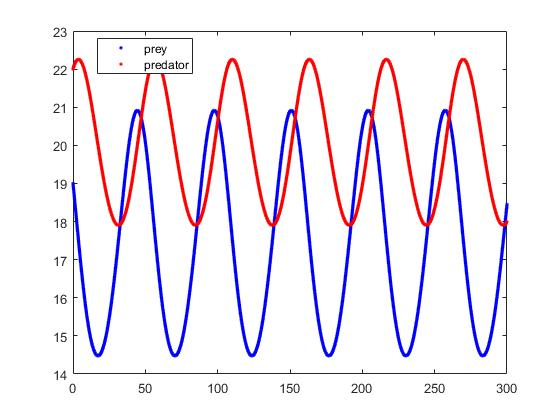
\includegraphics[width=.6\linewidth]{ex5.jpg}
				\caption{Evolution of the number of preys and predators.}
				\label{fig:ex5}
			\end{figure}
			
			Figure \ref{fig:ex5} shows the solution of these equations using the 4-th order Runge Kutta method explained before.
			The results are as expected. 
			The increase of the number of preys sustains the increase in the number of predators, the number of preys then reduce and consequently so does the numbers of predators due to less food avaulability.
			This is the explanation for the sinusoidal evolution of these values with the predator having a lower amplitude and being delayed relative to the prey evolution.
	
\end{document}



